\section{问题二的建模与求解}
\label{sec:problem2}

在问题一给出数据质量评分 $Q$ 与领域配比 $\boldsymbol{p}$ 之后，问题二需要把它们纳入同一损失模型。
本节先陈述广义标度律的形式及其设计约束，再说明数据条件所决定的参数辨识顺序；
随后依次报告三项预声明判据、质量指数的双路线结论、边际效用与等价条件，
以及域间关系与跨源迁移验证。
全节数值取源工件的落盘精度：参数与指数在正文中保留四位小数，
需与落盘表格逐位对照处保留八位，凡作四舍五入均在相应位置说明。

\subsection{广义标度律的形式与设计动机}
\label{subsec:q2-form}

经典标度律把损失分解为不可约项、容量项与数据项之和，见式~\eqref{eq:classic-law}。
数据质量与领域配比并不显式出现在其中，而二者恰是当前语料工程的主要着力点。
把质量作为独立加性项追加到~\eqref{eq:classic-law} 是最自然的写法，
但这样会破坏一项形式约束：当质量取参照值、配比取均匀时，模型不应残留任何与二者有关的分量。
本文因此采用乘性进入方式，把质量与配比都并入数据量项，得到

\begin{equation}
  L = E_s + A\,N^{-\alpha}
      + B\,\bigl(D\,Q^{\gamma}\exp(\boldsymbol{b}^{\top}\boldsymbol{z}_{\boldsymbol{p}})\bigr)^{-\beta},
  \label{eq:q2-generalized}
\end{equation}

其中 $E_s$ 为来源专属的不可约损失，$D_{\text{eff}}=D\,Q^{\gamma}\exp(\boldsymbol{b}^{\top}\boldsymbol{z}_{\boldsymbol{p}})$
为有效 token 数（effective token count），$\boldsymbol{z}_{\boldsymbol{p}}$ 为配比相对均匀配比的中心化偏离。
当 $Q=1$ 且 $\boldsymbol{z}_{\boldsymbol{p}}=\boldsymbol{0}$ 时，$Q^{\gamma}=1$、$\exp(\boldsymbol{0})=1$，
式~\eqref{eq:q2-generalized} 逐项退化为式~\eqref{eq:classic-law}。
这一退化性质是形式设计的硬约束，也是后文判据 1 的直接检验对象。

两种进入方式的语义并不相同，这是选择乘性写法的实质理由。
$Q^{\gamma}$ 表示质量对有效数据量的放大或折损，指数 $\gamma$ 刻画放大是否按比例：
$\gamma=1$ 时质量翻倍等价于 token 数翻倍，$\gamma<1$ 时质量的边际作用递减。
在数据受限条件下，重复使用同一批 token 的收益会随重复次数衰减，
该效应正是通过把重复次数折算为有效 token 数来刻画的\citep{muennighoff2023}；
数据修剪按信息量排序后保留子集，其效果同样可理解为改变了有效数据规模\citep{sorscher2022}。
领域配比则经 $\exp(\boldsymbol{b}^{\top}\boldsymbol{z}_{\boldsymbol{p}})$ 进入，
$\boldsymbol{b}=(b_1,\dots,b_{17})$ 由问题一配比模型的系数 $\theta_d$ 经中心化得到，即 $\boldsymbol{b}=\kappa(\boldsymbol{\theta}-\bar\theta)$，其中 $\kappa<0$。
中心化的作用有两个：均匀配比成为零点，从而与退化条件相容；
同时 $\boldsymbol{b}$ 的整体标度被吸收进系数 $B$，
使比值 $b_i/b_j$ 不依赖该标度，这一点在域间比较中会直接用到。
在 B6 半合成网格上，本文另比较了质量的乘性与加性两种规格，
二者的 RMSE 相对差为 0.035382，低于 10\% 的可区分阈值，数据本身无法在二者之间作出选择。
本文据此依形式约束选择乘性写法：加性形式在 $Q=1$ 处残留一项独立衰减，
与退化要求不相容。加性形式作为备用规格保留，其触发条件为 $\gamma$ 的区间含零或 B7 上不优于基线；
本轮两条条件均不成立，该规格保持休眠。

幂律形式本身的普适性不宜预设。已有工作指出标度指数并非先验常数，
其取值与数据流形的内在维度和目标的分解方式有关\citep{bahri2024}，
因此本文不把 $\alpha$、$\beta$ 视为已知常数，而作为待估参数并给出重抽样区间。
图~\ref{fig:q2-framework} 给出本问的建模与求解流程：
多源数据整备、退化检验、参数辨识（联合拟合）、跨源验证与条件化检验五个环节依次衔接，
末一环节由参数共享假设的检验结果触发。

\begin{figure}[htbp]
  \centering
  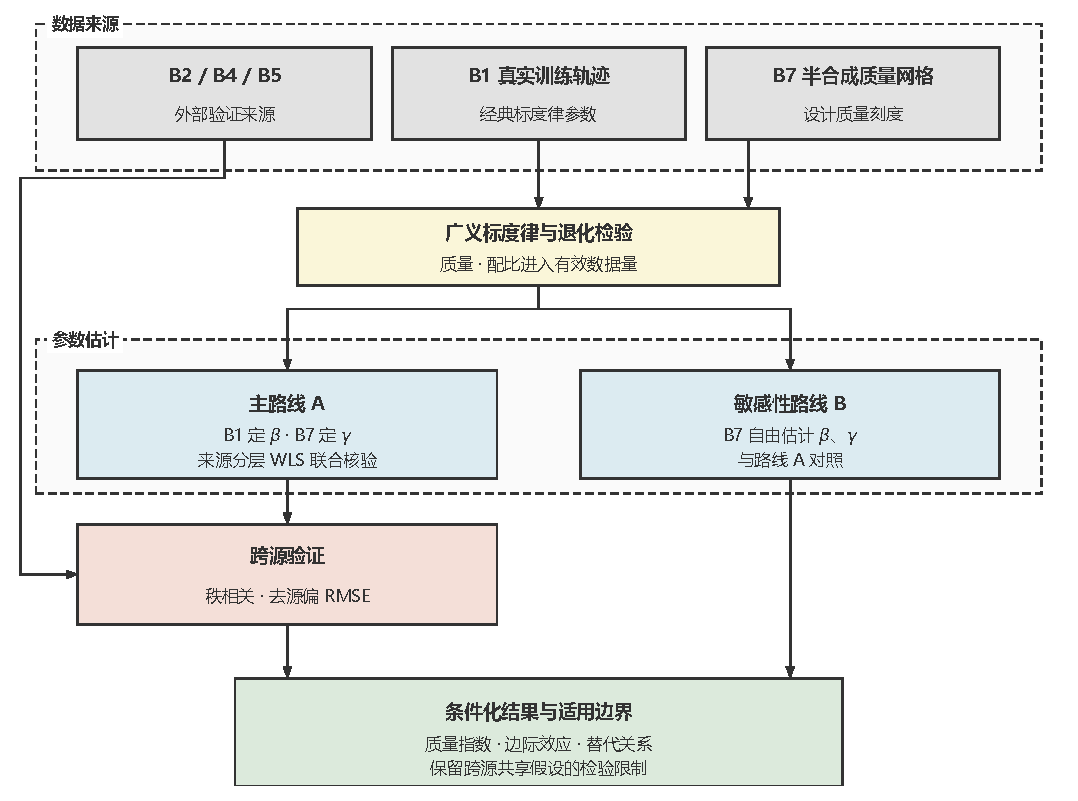
\includegraphics[width=0.96\linewidth]{figures/fig_framework_q2.pdf}
  \caption{问题二的建模与求解流程。上排五个环节依次为多源数据整备、退化检验、参数辨识（联合拟合）、
  跨源验证与条件化检验，下方汇文本问在质量指数上的两条路线结论及其区间，两路线的差别仅在于
  数据量指数的来源假设。}
  \label{fig:q2-framework}
\end{figure}

单位方面，$N$ 与 $D$ 均以十亿计，损失以 nats/token 计，$Q$ 无量纲且取值于 $(0,1]$。
数据量的量纲被系数 $B$ 与不可约项 $E_s$ 吸收，二者的数值随单位选择而变，
全文固定以十亿为单位报告。

\subsection{数据条件与参数辨识顺序}
\label{subsec:q2-identification}

可用数据对参数的支撑并不均衡，这直接决定了估计策略。
B1 为 Pythia 的真实训练轨迹\citep{biderman2023pythia}，
含 1176 行记录、8 个参数量取值，数据量跨 0.1--299.9B，
是附件中唯一同时含有 $N$、$D$ 变化且来自真实训练的轨迹。
质量因子的信息则只存在于 B6--B8 三个因子设计网格，三者均为半合成数据，
其中 B7 含质量取值 10 个、记录 450 行、参数量取值 9 个、数据量仅 5 个不同取值。
该网格兼具质量变化与半合成两重属性，凡建立在其上的结论都带补充分析的性质。

上述分布造成一项结构性限制：B1 上 $Q\equiv1$，对 $\gamma$ 不提供任何信息；
B7 上质量在设计网格内变动，但数据量只有 5 个不同取值，且与参数量在设计上相互纠缠。
换言之，数据量指数与质量指数无法在同一份数据上同时获得良好辨识。
本文因此固定估计顺序：先由真实轨迹 B1 反解数据量指数 $\beta$，
再在 B7 上以该 $\beta$ 反解 $\gamma$，而各来源的形状参数分别独立估计。
该顺序的代价是 $\gamma$ 的精度部分继承自 $\beta$，
本文把这一依赖作为独立的可检验命题处理，结果见 \S\ref{subsec:q2-conditional}。

\begin{table}[htbp]
  \centering
  \caption{广义标度律与基线的参数估计（$N$、$D$ 以十亿计，损失以 nats/token 计）}
  \label{tab:q2-params}
  \begin{tabular}{@{}lccc@{}}
    \toprule
    参数 & 基线 M0s（B1） & 主方法 M1s（B1 侧） & 主方法 M1s（B7 侧） \\
    \midrule
    $E_s$      & 1.68979756 & 1.68979741 & 1.65423173 \\
    $A$        & 0.35398032 & 0.35398032 & 0.52912380 \\
    $\alpha$   & 0.33997658 & 0.33997658 & 0.28321756 \\
    $B$        & 1.24030558 & 1.24030577 & 1.05387051 \\
    $\beta$    & 0.27987813 & \multicolumn{2}{c}{0.27987806（跨源共享）} \\
    $\gamma$   & ---（不含质量项） & ---（B1 上 $Q\equiv1$） & 0.96591294 \\
    \bottomrule
  \end{tabular}
\end{table}

表~\ref{tab:q2-params} 列出两套参数与基线。基线 M0s 取经典形式~\eqref{eq:classic-law} 并仅用 B1 拟合。
主方法与基线在 B1 侧的形状参数在数值上近乎重合：$A$ 与 $\alpha$ 逐位相同，
$E_s$ 与 $B$ 的相对差约 $10^{-7}$，差异仅出现在第八位有效数字，
其原因是质量项与配比项在 $Q=1$、$\boldsymbol{z}_{\boldsymbol{p}}=\boldsymbol{0}$ 处恰取单位元。
B7 侧的形状参数与 B1 侧差异明显：$A$ 的比值为 1.4948，$B$ 为 0.8497，
$\alpha$ 由 0.33997658 变为 0.28321756。
形状参数能否跨源共享因此需要单独检验。强制 $A$、$\alpha$、$B$ 跨源共享，
会使 $\gamma$ 位移 0.169104，即其重抽样区间宽度的 0.9850 倍，远超预声明的 50\% 阈值，
共享在 B7 上另带来 0.015493 的 RMSE 代价。
本文据此把形状参数设为来源专属，并如实报告这一结构的后果：
在来源专属的形状参数下，加权最小二乘的联合求解在数值上退化为
「由 B1 定 $\beta$、由 B7 定 $\gamma$」的两段式，
实测两段式解与联合解在 $\gamma$ 上相差 $1.03\times10^{-7}$、在 $\beta$ 上相差 $6.86\times10^{-8}$。
权重机制被完整实现，但在该参数结构下不产生可分辨的修正，
因此本节不以联合拟合作为估计精度的来源。

分层权重由各来源的拟合残差估计，得 $\sigma_{B1}=1.465\times10^{-4}$、$\sigma_{B7}=0.076384$，
逐点权重比为 $3.678\times10^{-6}$，B7 在联合目标中的总权重份额为 $1.408\times10^{-6}$。
需要说明，本轮的分层权重取残差口径，该选择尚未经独立确认；
其消融检验（改用另一锚点口径）给出 $\gamma$ 的位移为 0.000341，小于区间宽度，
故结论对权重口径不敏感。

\subsection{三项预声明判据与判据的替换}
\label{subsec:q2-criteria}

主方法的评价不以拟合优度的直观好坏为准，而以实验前声明的三项判据为准，
阈值、实测与结论列于表~\ref{tab:q2-criteria}。

\begin{table}[htbp]
  \centering
  \caption{三项预声明判据的阈值、实测值与结论}
  \label{tab:q2-criteria}
  \begin{tabular}{@{}>{\raggedright\arraybackslash}p{0.17\linewidth}>{\raggedright\arraybackslash}p{0.20\linewidth}>{\raggedright\arraybackslash}p{0.40\linewidth}>{\raggedright\arraybackslash}p{0.09\linewidth}@{}}
    \toprule
    判据 & 预声明阈值 & 实测 & 结论 \\
    \midrule
    1 退化检验（B1） & RMSE 相对差 $<10^{-6}$ &
      $1.0122\times10^{-8}$（基线 0.0001464960899 对主方法 0.0001464960914） & 通过 \\
    2 超越性（B7） & RMSE 降幅的自助 95\% 区间不含零 &
      降幅 0.041868，区间 $[0.036236,0.047781]$（由 0.118252 降至 0.076384） & 通过 \\
    3 弹性符号 & 三个弹性均为负 & B1 侧与 B7 侧均成立 & 通过 \\
    \bottomrule
  \end{tabular}
\end{table}

判据 1 检验退化性质。在 B1 上，主方法与基线的 RMSE 相对差为 $1.0122\times10^{-8}$，
低于 $10^{-6}$ 阈值，该量级表明二者的差异已落进数值精度。
此处须辨明该判据的角色：它检验的是 $Q=1$、$\boldsymbol{z}_{\boldsymbol{p}}=\boldsymbol{0}$ 时
模型是否退回经典形式，而不是主方法相对基线的性能比较。
在 B1 上二者本应同形同自由度，任何性能差异都不构成改进的证据，
该判据的双重作用在于它同时也是题目所要求的退化性质的依据。

判据 2 检验超越性，在 B7 上进行。不含质量项的基线在该网格上的 RMSE 为 0.118252，
主方法为 0.076384，降幅 0.041868，自助 95\% 区间 $[0.036236,0.047781]$ 不含零。
该比较的两个对象在 B7 上各自设有来源专属截距，这是不可约损失不可跨源共享的机械后果；
若改用 B1 的截距预测 B7，截距失配会被计入质量通道的贡献。
判据 3 检验弹性（elasticity）符号：$\partial L/\partial N$、$\partial L/\partial D$、$\partial L/\partial Q$
在 B1 侧与 B7 侧均为负，与「增加任一资源要素都降低损失」的机理一致。

判据的形式在代码生成之前经过一次修正，其对象与时序须一并交代。
方法卡原预声明的第 1 条判据为「主方法在 B1 留出集上的 RMSE」，
但该判据在本数据条件下结构性失效：B1 不含配比列，故 $\boldsymbol{z}_{\boldsymbol{p}}=\boldsymbol{0}$、
$\exp(\boldsymbol{b}^{\top}\boldsymbol{z}_{\boldsymbol{p}})=1$；
B1 又不含质量变化，故 $Q$ 为常数，$Q^{\gamma}$ 并入系数 $B$。
两项叠加，主方法在 B1 上塌缩为与基线同形、同自由度的模型，
留出集 RMSE 不可能给出任何关于质量通道的信息。
本文因此把第 1 条改为退化检验，把超越性比较移到 B7。
该修正发生在代码生成之前，方向是收紧而非放宽：
它撤销了原判据本可提供的、形式上更有利但内容为空的比较，
并把质量通道的举证责任集中到唯一含质量变化的网格上。
该修正的方向与本节其余判据的收紧方向一致，不构成对判据的事后放宽。

\subsection{质量指数的双路线结论与参数共享检验}
\label{subsec:q2-conditional}

$\gamma$ 的取值依赖 $\beta$ 的来源假设，二者不能分开报告。
在 B7 的设计刻度上、且 $\beta$ 取自 B1（0.279878）时，
$\gamma=0.965913$，自助（bootstrap）95\% 区间 $[0.883860,1.055546]$ 含 1.0，
据此 $D_{\text{eff}}\approx D\,Q$，质量的相对变化按比例放大有效 token 数。
若 $\beta$ 改在 B7 上自由估计，$\gamma=1.179781$，区间 $[1.088441,1.283359]$ 不含 1.0，
此时质量的放大作用略强于按比例。两条路线并列见图~\ref{fig:q2-gamma-routes}。

\begin{figure}[htbp]
  \centering
  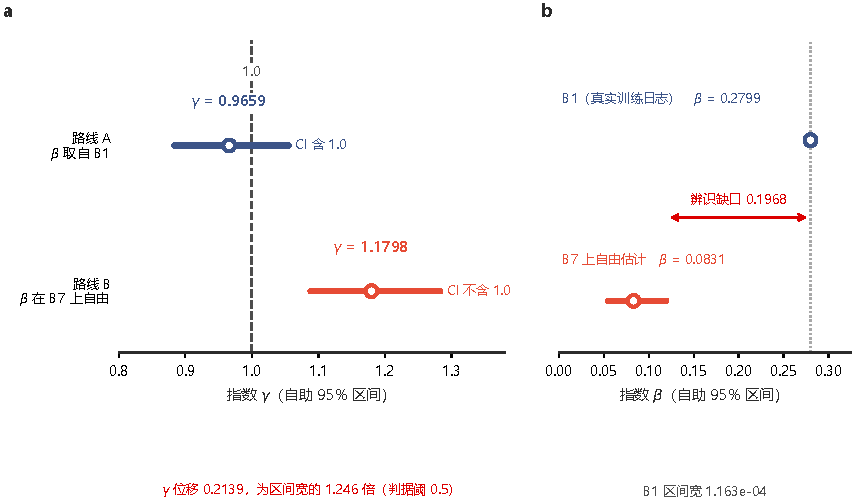
\includegraphics[width=0.92\linewidth]{figures/fig_q2_gamma_routes.pdf}
  \caption{质量指数 $\gamma$ 的两条路线与数据量指数 $\beta$ 的辨识缺口。
  (a) 路线 A（$\beta$ 取自 B1）与路线 B（$\beta$ 在 B7 上自由估计）的 $\gamma$ 点估计与自助 95\% 区间，
  虚线为 $\gamma=1$；两条区间的交叉与否决定了有效 token 数是否按比例放大。
  (b) 两条路线下 $\beta$ 的估计与区间，二者的区间不重叠。
  横轴为指数取值，纵轴为路线。}
  \label{fig:q2-gamma-routes}
\end{figure}

两条路线的 $\gamma$ 位移为 0.213868，等于其自助区间宽度的 1.245692 倍，
超过预声明的 0.5 阈值，故「$\beta$ 可跨源共享」这一假设在本文判据下未获通过；
与之相伴，两条路线的 $\beta$ 互不覆盖：B7 自由估计给出 $0.083064$（区间 $[0.054791,0.119420]$），
而 B1 的 $\beta=0.279878$ 落在该区间之外。
放开 $\beta$ 还使 B7 的 RMSE 由 0.076384 降到 0.069544，改善约 9\%，
说明共享 $\beta$ 是一项真实约束而非平坦方向。

本文仍取 B1 的 $\beta$，理由是辨识强度：B1 的 $\beta$ 区间宽度仅 $1.163\times10^{-4}$，
其 1176 行数据的数据量跨 0.1--299.9B；B7 只有 5 个不同的数据量取值，
且与参数量在设计上纠缠，$\beta$ 的独立辨识条件明显更弱。
该理由只说明当前取值在估计效率上的依据，并不构成上述检验未发生的理由。
该检验未通过这一事实意味着 $\gamma\approx1$ 是条件性结论而非无条件实测结论，
下文凡含 $\gamma$ 的量都继承该条件。
另一种规避条件性的做法是改报乘积 $\beta\gamma$，但条件性并不会因此消失：
按两条路线各自的 $\beta$ 与 $\gamma$ 计算，该乘积分别为 0.2703 与 0.0980，相差 2.76 倍，
其路线依赖比 $\gamma$ 本身更强，故本节不作此替换。

\subsection{边际效用、弹性与等价条件}
\label{subsec:q2-marginal}

在同一参照点 $N=1.0$B、$D=150.0$B、$Q=0.5$ 上计算偏导与弹性，结果列于表~\ref{tab:q2-elasticity}。
两侧同报是因为数据的支撑性质不同：$\partial L/\partial N$、$\partial L/\partial D$
及其弹性可由 B1 的真实轨迹支撑，而含 $\gamma$ 的量
（$\partial L/\partial Q$、质量弹性、替代率与等价补偿量）不可避免地依赖半合成网格 B7。
两侧量级的相对差为 15.0\%--31.8\%，该差可视为配比与质量的效应形状
跨来源迁移这一假设的代价的量化。

\begin{table}[htbp]
  \centering
  \caption{参照点 $N=1.0$B、$D=150.0$B、$Q=0.5$ 处的边际效用、弹性与等价条件}
  \label{tab:q2-elasticity}
  \begin{tabular}{@{}lccc@{}}
    \toprule
    量 & B1 侧（主） & B7 侧（敏感性） & 相对差 \\
    \midrule
    $\partial L/\partial N$            & $-0.120345$ & $-0.149857$ & 0.2452 \\
    $\partial L/\partial D$            & $-0.000687$ & $-0.000583$ & 0.1503 \\
    $\partial L/\partial Q$            & $-0.198978$ & $-0.169069$ & 0.1503 \\
    $N$ 的弹性                          & $-0.120345$ & $-0.149857$ & --- \\
    $D$ 的弹性                          & $-0.103000$ & $-0.087518$ & --- \\
    $Q$ 的弹性                          & $-0.099489$ & $-0.084534$ & --- \\
    $Q\!\to\!N$ 替代率                  & $-1.653397$ & $-1.128200$ & 0.3176 \\
    $Q$ 增 $0.1$ 的 $N$ 补偿量/B        & $-0.134101$ & $-0.094469$ & 0.2955 \\
    $Q$ 弹性与 $D$ 弹性之比             & 0.96591294  & 0.96591294  & 0.0000 \\
    \bottomrule
  \end{tabular}
\end{table}

题目要求的等价条件以「质量增加 0.1 所需的参数量补偿」表达。
在给定参照点下，B1 侧为 $-0.134101$B，B7 侧为 $-0.094469$B；
符号为负表示提高质量可以减少所需参数量。
该量必须与参照点一同理解：偏导随位置变化，脱离参照点的量级没有意义。
就量级而言，该结论与语料治理的已有证据方向一致：
在大规模网络语料上做质量筛选后，同等训练预算下的损失明显低于未筛选的对照，
筛选带来的收益可与扩大数据规模部分互换\citep{penedo2024fineweb}。

弹性之间存在一条恒等式，它决定了哪些替代关系可以谈。
在 $D_{\text{eff}}=D\,Q^{\gamma}$ 的设定下，质量弹性与数据量弹性之比恒等于 $\gamma$，
两侧相对差为 0.0000，实测极差小于 $10^{-12}$，
即该比值随位置保持不变，它只是 $\gamma$ 的另一种读法。
因此在本文模型下，随位置变化的只有 $Q$ 与 $N$ 之间的替代率；
$Q$ 与 $D$ 之间的替代率是常数。这一区分影响解读：
以质量替换数据量本身不存在位置相关的换算关系，而以质量替换参数量则存在。

\subsection{域间关系与跨源迁移验证}
\label{subsec:q2-domain}

$\boldsymbol{b}$ 的绝对量级在附件 B 上不可辨识，实测 RMSE 随标度常数 $\kappa$ 的变化恰为零。
本节因此只报各域相对参照域 \texttt{train\_the\_pile\_philpapers} 的比值与符号，
17 个域的取值见图~\ref{fig:q2-domain-ratio}。
参照域取值为 1.000000，其损失水平最高；
\texttt{dm\_mathematics} 为 $-1.618816$，是全表唯一 $|b_i/b_{\text{ref}}|>1$ 的域；
其余 15 个域的绝对值均不超过 1。
该比值的语义需要说明：它是中心化权重之比而非有界比例，
负值只表示上调该域会降低损失，与参照域方向相反，不能读作损失本身为负。
这 17 个域的划分以 Pile 语料的领域定义为基础\citep{gao2020pile}，
其相对排序与领域间配比优化的已有观察方向一致：
领域之间存在结构性差异，最优权重取决于领域的语言性质与目标任务的匹配程度，
故配比在较小尺度上的回归预测\citep{liu2024regmix}与训练过程中的动态调整\citep{xie2023doremi}
都以图~\ref{fig:q2-domain-ratio} 给出的域间排序为共同前提。

\begin{figure}[htbp]
  \centering
  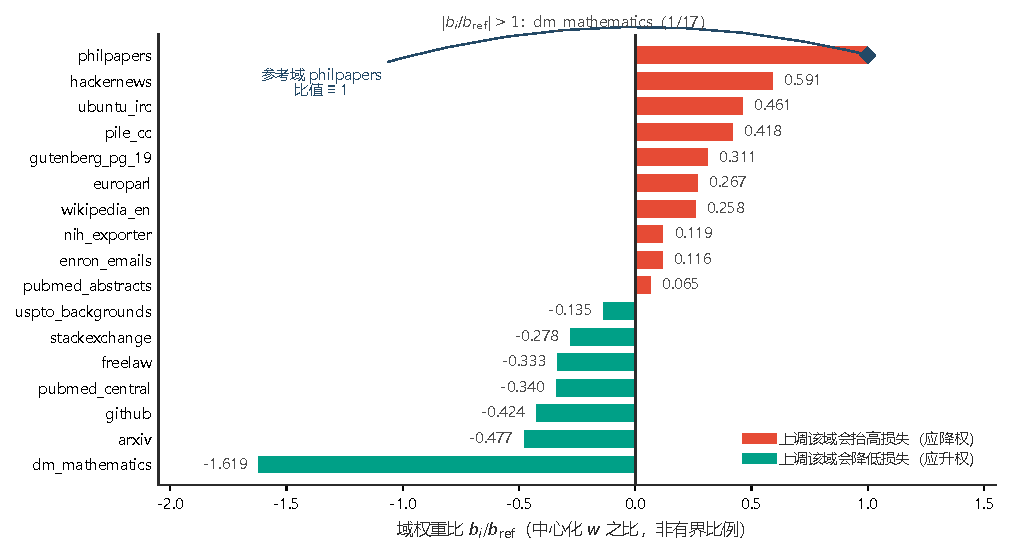
\includegraphics[width=0.92\linewidth]{figures/fig_q2_domain_ratio.pdf}
  \caption{17 个训练领域相对参照域 \texttt{train\_the\_pile\_philpapers} 的权重比 $b_i/b_{\text{ref}}$，
  按取值降序排列。横轴为中心化权重之比（非有界比例），纵轴为领域名；
  正负分别对应上调该域会抬高与降低损失。\texttt{dm\_mathematics} 为唯一绝对值超过 1 的域。}
  \label{fig:q2-domain-ratio}
\end{figure}

若要把 $\boldsymbol{b}$ 与 $N$、$D$、$Q$ 放在同一绝对尺度上比较，则需要引入 $\kappa$，
而 $\kappa$ 的取值随参照点变化：在 B1 的 1B 尺度运行内即从 $-14.215132$ 变到 $-1.6413$，相差 8.7 倍。
敏感性臂在数据量参照点 299.893B 上给出 $\kappa=-14.215132$、
$\boldsymbol{b}$ 的取值范围 $[-21.626478,35.009297]$，
以及把最低权重域调到最高权重域一个百分点所对应的损失变化 0.039842。
这些绝对量级只在对应参照点上成立，不存在普适取值。
更准确的表述是：$\boldsymbol{b}$ 内部相比与 $\kappa$ 无关，
$\boldsymbol{b}$ 与 $N$、$D$、$Q$ 相比则一定含 $\kappa$，
这正是配比的绝对效应无法跨源辨识的精确含义。

跨源迁移验证在三个外部来源上独立进行，结果见图~\ref{fig:q2-cross-source-validation}（a）。
B4 为跨模型族的收敛点，属真实观测，$n=57$，去源偏后的秩相关（rank correlation）为 0.982982；
B5 为文献报告的标度律数值，属他人发表而非本队观测，$n=44$，秩相关为 0.958808；
B2 为经真实数据校准并注入噪声的半合成轨迹，$n=1029$，秩相关为 0.788102。
三者的去源偏 RMSE 分别为 0.192657、0.199662 与 0.418526。
各来源的不可约损失差异悬殊，逐源拟合的 $E_s$ 极差达 1.689798，
故跨源未去偏的决定系数没有解释意义，本节只报秩相关与去源偏 RMSE。
其中 B2 的秩相关建立在半合成轨迹之上，不构成直接观测的迁移验证；
B5 的数值来自已发表文献，与本文实测结果的性质不同。
图~\ref{fig:q2-cross-source-validation}（b）另给出各边际效用两侧取值的对照，
其中 $Q$ 通道的量明确依赖半合成网格，符号一致性是它们可以承担的全部结论。

\begin{figure}[htbp]
  \centering
  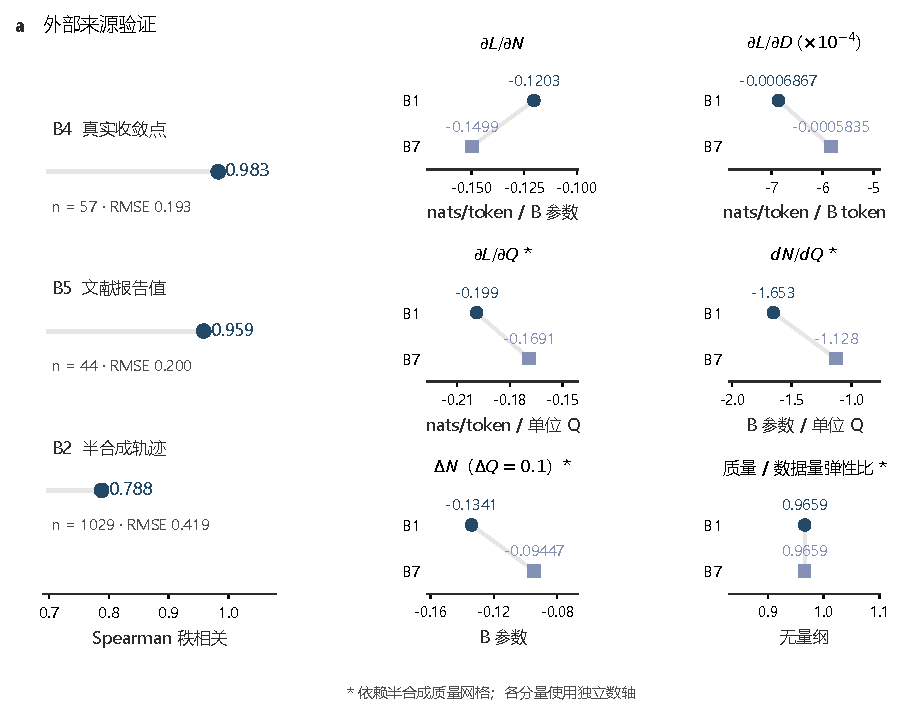
\includegraphics[width=0.92\linewidth]{figures/fig_q2_cross_source_validation.pdf}
  \caption{跨源迁移验证与弹性对照。
  (a) 三个外部来源的去源偏秩相关：B4（真实收敛点，$n=57$）、
  B5（已发表文献值，$n=44$）、B2（半合成轨迹，$n=1029$），
  点旁标注各自的去源偏 RMSE，横轴为 Spearman 秩相关。
  (b) 各边际效用在 B1 侧与 B7 侧的取值对照，星号标出无真实数据支撑、
  依赖半合成网格的量，横轴为对 $L$ 的偏导。}
  \label{fig:q2-cross-source-validation}
\end{figure}

余下是三项必须在结论中携带的限制。
其一，配比效应的可迁移性无法在本数据上检验：全部 11 个 B 类文件中无一含配比列（0/11），
因而不存在配比列与 $(N,D)$ 的联合读数；
问题一的三个训练尺度中也只有一个落入 B1 的参数量区间 $[0.070542,11.965825]$B。
该假设承重且不可检验，本问关于配比的全部结论都在其下成立。
其二，质量刻度的对齐尚未解决：问题一给出的经验域级质量落在 $[0.223306,0.381496]$，
而 B7 的设计网格取值为 $\{0.1,0.2,\dots,1.0\}$，二者不是同一对象。
本文不对二者作隐式映射，$\gamma$ 的数值解释因此绑定在 B7 的设计刻度上，
不能直接代入问题一的经验质量。
其三，B7 的生成过程与质量因子之间是否存在循环性尚未核验，
该不确定性一并声明，不影响上述形式结论，但影响 $\gamma$ 的绝对解释。

另需说明的是，B1 侧的拟合异常干净，$R^2=0.9999998$、RMSE $=1.465\times10^{-4}$，
对真实训练日志而言并不寻常。本文对该数据的处理附有一项谨慎要求，
相关核验尚未完成，故以 B1 为一侧参照的结论须在该要求下理解。
扰动检验显示结论对 B1 权重的依赖有限：
把 B1 在联合目标中的整体权重在 0.5 至 2 倍之间变动，$\gamma$ 的最大位移为 0.039812，
约为其区间宽度的 23\%；逐组留一数据量分组的 $\beta$ 极差为 $3.535\times10^{-5}$，
小于其区间宽度。这并不替代对 B1 处置方式的判断，只是说明本文结论对该处置不敏感。
